\documentclass[10pt,twocolumn,twoside]{article}

\usepackage[margin=0.72in,columnsep=0.26in]{geometry}
\usepackage[T1]{fontenc}
\usepackage[utf8]{inputenc}
\usepackage{lmodern}
\usepackage{microtype}
\usepackage{booktabs}
\usepackage{tabularx}
\usepackage{graphicx}
\usepackage{xcolor}
\usepackage{amsmath}
\usepackage{enumitem}
\usepackage{caption}
\usepackage{fancyhdr}
\usepackage{hyperref}
\usepackage{tikz}
\usepackage{flushend}
\usetikzlibrary{arrows.meta,positioning,shapes.misc}

\definecolor{navy}{HTML}{17324D}
\definecolor{teal}{HTML}{1D7A7A}
\definecolor{pale}{HTML}{EEF5F5}
\definecolor{warn}{HTML}{FFF4D6}
\definecolor{rulegray}{HTML}{CBD5DC}

\hypersetup{
  colorlinks=true,
  linkcolor=navy,
  citecolor=teal,
  urlcolor=teal,
  pdftitle={When GPUs Do Not Perform Best},
  pdfsubject={Pre-results study design for UAD-2 OCTO and GPU comparison}
}

\captionsetup{font=small,labelfont={bf,color=navy}}
\setlist{nosep,leftmargin=*}
\setlist[description]{style=multiline,leftmargin=24mm,labelwidth=21mm}
\setlength{\parindent}{0.9em}
\setlength{\parskip}{0pt}
\setlength{\columnsep}{0.26in}
\setlength{\headheight}{20pt}
\raggedbottom
\renewcommand{\arraystretch}{1.13}

\pagestyle{fancy}
\fancyhf{}
\fancyfoot[CO,CE]{\small\thepage}
\renewcommand{\headrulewidth}{0pt}
\fancypagestyle{plain}{%
  \fancyhf{}
  \fancyfoot[CO,CE]{\small\thepage}
  \renewcommand{\headrulewidth}{0pt}
}

\newcommand{\statusbox}[1]{%
  \begin{center}
  \colorbox{warn}{\parbox{0.94\textwidth}{\small\textbf{Evidence status.} #1}}
  \end{center}
}

\newcommand{\researchq}[1]{\textbf{RQ#1.}}

\begin{document}

\twocolumn[
\begin{@twocolumnfalse}
  \begin{center}
    {\color{navy}\LARGE\bfseries When GPUs Do Not Perform Best\par}
    \vspace{0.2em}
    {\large Evaluating UAD-2 OCTO DSPs for Low-Latency Streaming Workloads\par}
    \vspace{0.65em}
    {\small Pre-results manuscript and experimental protocol, August 2026\par}
  \end{center}

  \begin{abstract}
  Modern graphics processors provide exceptional throughput when a workload
  exposes enough parallel work to amortize launch, synchronization, and data
  movement. Real-time audio and other streaming workloads often occupy the
  opposite regime: small buffers, persistent state, serial dependencies, and
  hard deadlines. This paper asks where an eight-DSP UAD-2 OCTO accelerator
  can outperform a commodity discrete GPU when performance is defined by
  end-to-end latency, tail latency, deadline misses, throughput, and energy,
  rather than peak floating-point rate alone. We specify matched workloads,
  correctness requirements, optimized baselines, measurement procedures, and
  a decision rule for identifying crossover regions. The present UAD stack
  initializes all command and response rings, starts all eight DSP engines,
  and recovers each engine independently, but it has not yet completed a
  general-purpose program. Therefore, this version is a study design and does
  not claim a measured UAD performance advantage. Its central contribution is
  a falsifiable protocol that can support such a claim if, and only if, the
  resulting data satisfy the preregistered criteria.
  \end{abstract}

  \statusbox{The repository contains no completed UAD program and no GPU
  benchmark. All comparative outcomes in this manuscript are hypotheses. A
  results paper must replace this status with correctness-checked measurements.}
  \vspace{0.6em}
\end{@twocolumnfalse}
]

\section{Introduction}

GPUs are designed to sustain high throughput across many concurrent threads.
That design is compelling for large matrices, long convolutions, and highly
parallel physical models. It does not imply that a GPU minimizes the completion
time of every job. NVIDIA's own optimization guidance emphasizes that
host-device transfers must be included in application timing and that many
small transfers should be batched \cite{nvidia-best-practices}. Those costs are
especially relevant when a real-time system must process a small buffer and
return it before the next buffer arrives.

Prior audio-GPU studies already suggest a crossover rather than a universal
winner. Renney, Mitchell, and Gaster reported a hardware-dependent baseline GPU
overhead near 0.1 ms and found that feasible buffer sizes depended on sample
rate, latency, and jitter constraints \cite{renney2020}. A later comparison of
CPU, GPU, and FPGA implementations of modal reverberation showed both the very
high throughput available from a GPU and meaningful variation in per-buffer
latency \cite{michon2025}. These findings motivate a workload-centered study.

The target platform is a Universal Audio UAD-2 OCTO PCIe card. Universal Audio
describes the OCTO as an eight-SHARC accelerator \cite{ua-uad2-pcie}. Static and
high-resolution optical evidence confirms all eight processors as
ADSP-21469 KBCZ-00 devices, for which Analog Devices specifies up to a
450 MHz floating-point core and 2700 MFLOP/s peak performance per processor
\cite{adi-adsp21469}. Peak rates alone are not the proposed advantage. The
hypothesis is that persistent DSP state, audio-oriented execution, and
independent engines may benefit small, deadline-sensitive streams.

This study is designed to make that hypothesis difficult to confirm by accident.
It compares equivalent numerical work, includes optimized GPU paths, reports
tail behavior rather than averages alone, and includes workloads expected to
favor the GPU. The intended contribution is a map of the crossover boundary,
not a collection of hand-picked wins.

\paragraph{Contributions after execution is available.}
The completed paper is intended to provide:

\begin{enumerate}
  \item a reproducible UAD-2 OCTO execution path with bounded DMA,
  correctness checking, and per-DSP recovery;
  \item matched UAD, GPU, and reference CPU implementations of small streaming
  kernels and high-parallelism controls;
  \item end-to-end latency distributions, deadline-miss rates, throughput,
  energy, and one-to-eight-DSP scaling; and
  \item an explicit crossover map over buffer size, channel count, workload
  statefulness, and GPU contention.
\end{enumerate}

At present, only the first contribution's transport and empty-engine recovery
components are established \cite{uad-project}.

\section{Research Questions and Claims}

\researchq{1} For which combinations of buffer size, channel count, and kernel does
the UAD have lower end-to-end p99 latency than an optimized discrete GPU?

\researchq{2} At a fixed audio deadline, which platform has the lower miss rate and
smaller worst-case scheduling jitter?

\researchq{3} Where does the UAD provide lower energy per correct output buffer, and
does that conclusion survive idle-power subtraction and uncertainty analysis?

\researchq{4} How does throughput scale from one to eight independent UAD DSPs, and
what shared transport bottlenecks limit that scaling?

\researchq{5} At what point do increasing arithmetic intensity and parallelism make
the GPU the unambiguous winner?

The primary hypothesis is narrow: the UAD may win for small, stateful,
deadline-sensitive streams whose work cannot fully occupy a GPU. The reciprocal
hypothesis is equally important: a GPU should win as buffers, independent
channels, filter length, or model size increase. A credible paper must report
both regions.

\section{Tested Platform and Current Evidence}

\begin{figure*}[t]
  \centering
  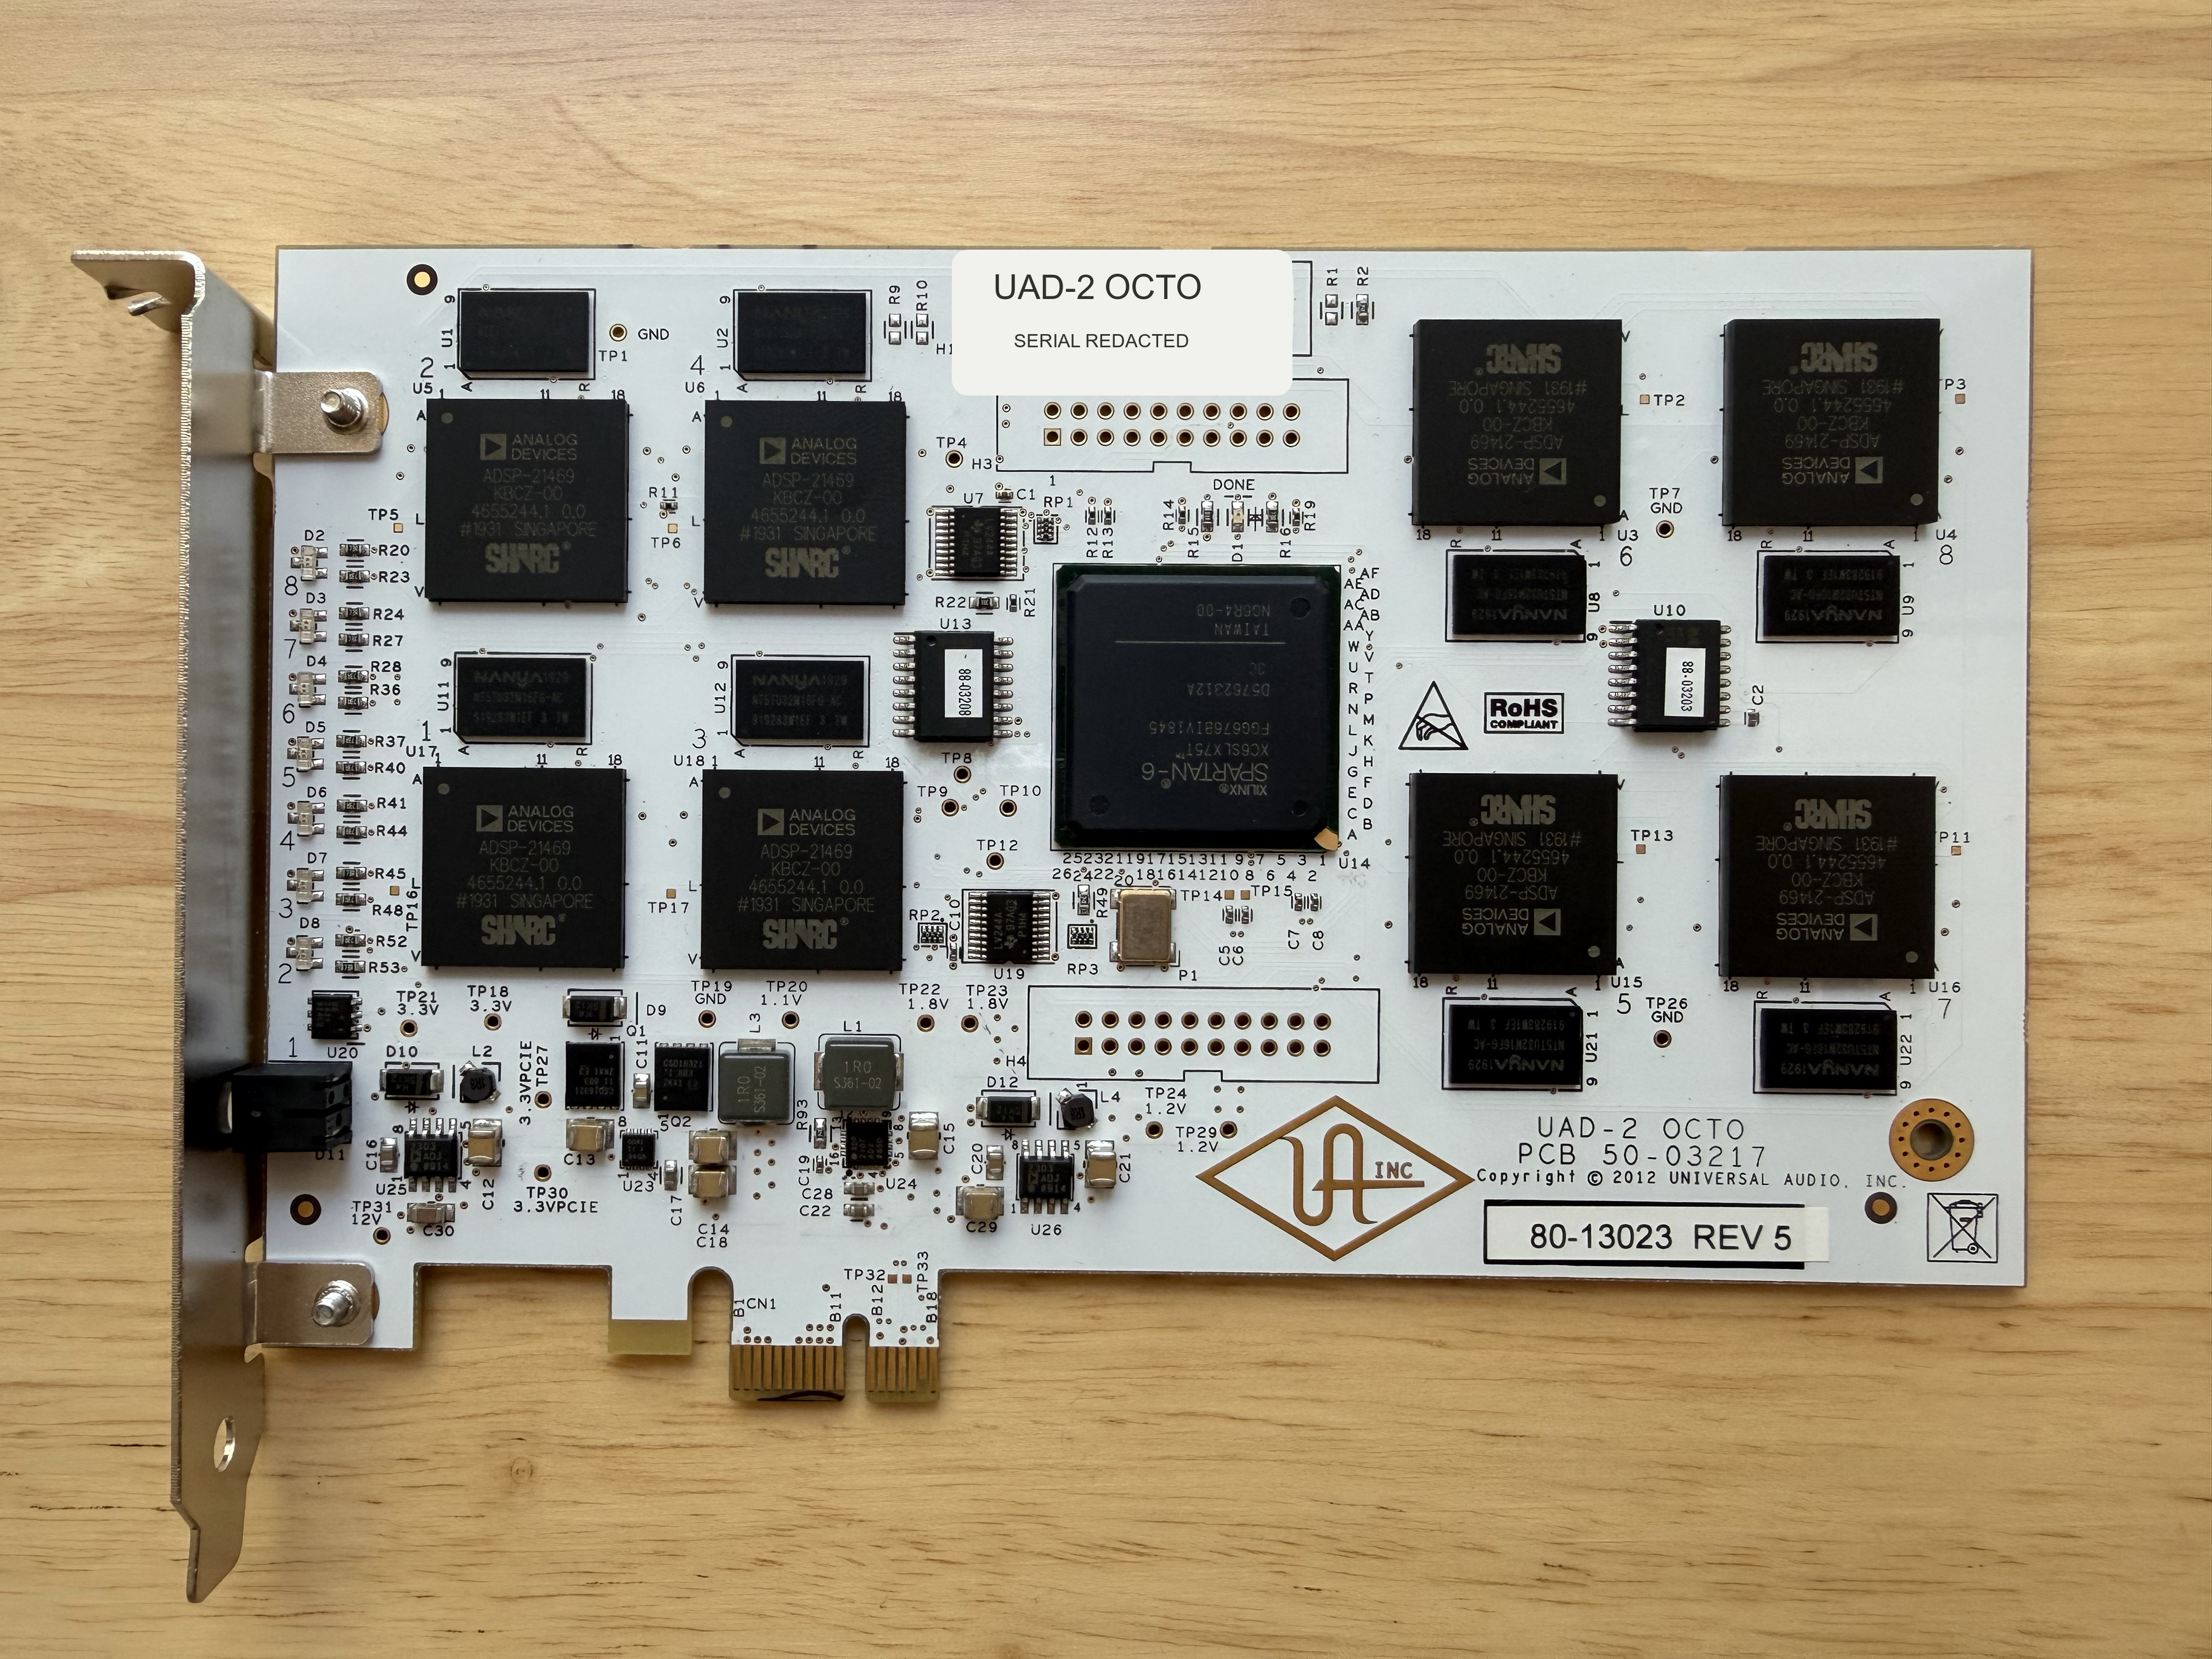
\includegraphics[width=0.95\textwidth]{../docs/images/uad2-octo-rev5-highres.jpg}
  \caption{The UAD-2 OCTO Rev. 5 board used by the project. The photograph
  optically resolves all eight ADSP-21469 KBCZ-00 SHARC packages and the
  central XC6SLX75T FGG676 Spartan-6 FPGA. The serial-label area is redacted in
  the public artifact.}
  \label{fig:board}
\end{figure*}

The tested endpoint reports PCI identity \texttt{1a00:0002}, subsystem
\texttt{1a00:0005}, a 64 KiB BAR, a PCIe 2.5 GT/s x1 link, and eight DSP-ready
locations. The reverse-engineered host path publishes 16 command and response
rings using 64 IOMMU-contained pages. It can start all eight engines and reset
each empty engine independently. These observations are tied to one Rev. 5
card and should not be generalized to older UAD-2 endpoints.

Table~\ref{tab:evidence} separates transport evidence from performance evidence.
The distinction is essential: a moving ring index proves dequeue behavior, not
correct program execution or low latency.

\begin{table*}[t]
\centering
\caption{Evidence available before the proposed benchmark campaign.}
\label{tab:evidence}
\small
\begin{tabularx}{0.97\textwidth}{@{}p{0.22\textwidth}p{0.16\textwidth}X@{}}
\toprule
Capability & Status & Interpretation \\
\midrule
Exact PCI endpoint and isolated IOMMU group & Confirmed & The tested card can be identified and its DMA can be contained. \\
All-eight ring and DMA transport startup & Confirmed & All 16 rings and 64 pages can be published and recovered. \\
Per-DSP reset on an empty transport & Confirmed & Each engine can be pulsed and returned to its baseline without changing the other seven. \\
Valid runtime response & Not observed & Official commands dequeue, but no response has been received. \\
General-purpose program and bounded output & Not achieved & No UAD workload can yet be compared for correctness or speed. \\
GPU baseline and comparison dataset & Absent & No GPU model, CUDA stack, timing distribution, power trace, or result file exists. \\
\bottomrule
\end{tabularx}
\end{table*}

The processor identification is now direct at the component level. All eight
packages visibly carry \texttt{ADSP-21469} and \texttt{KBCZ-00}; the central
FPGA visibly carries \texttt{XC6SLX75T} and \texttt{FGG676}. The Analog Devices
data sheet identifies the processor package as a 324-ball CSP\_BGA and specifies
up to 450 MHz, while AMD lists the observed FPGA/package combination
\cite{adi-adsp21469,amd-spartan6-packaging}. The DSP speed ordering suffix is
not visible, so the exact board clock remains unmeasured.

\section{Comparison Model}

\begin{figure*}[t]
\centering
\begin{tikzpicture}[
  node distance=8mm and 12mm,
  box/.style={draw=navy,rounded corners=2pt,fill=pale,minimum height=8mm,
              minimum width=27mm,align=center,font=\small},
  metric/.style={draw=teal,rounded corners=2pt,fill=white,minimum height=8mm,
                 minimum width=35mm,align=center,font=\small},
  arr/.style={-{Latex[length=2mm]},thick,color=navy}
]
\node[box] (input) at (0,0) {Pinned host input\\and timestamp};
\node[box] (uad) at (4.0,0.75) {UAD path\\ring, DMA, DSP};
\node[box] (gpu) at (4.0,-0.75) {GPU path\\copy, launch, kernel};
\node[box,minimum width=38mm] (output) at (8.5,0) {Verified host output\\and completion timestamp};
\node[metric] (metrics) at (13.3,0) {Latency distribution\\deadline misses\\throughput and energy};
\draw[arr] (input.east) -- (uad.west);
\draw[arr] (input.east) -- (gpu.west);
\draw[arr] (uad.east) -- (output.west);
\draw[arr] (gpu.east) -- (output.west);
\draw[arr] (output.east) -- (metrics.west);
\end{tikzpicture}
\caption{Primary end-to-end comparison. Timing begins before platform
submission and ends only after the output is visible to the host and verified.
Device-only timing is reported separately and cannot replace this path.}
\label{fig:model}
\end{figure*}

The primary comparison is host-visible, end-to-end completion, as shown in
Figure~\ref{fig:model}. Both platforms receive the same input samples and
produce the same output layout. Timing includes every operation required for
the host to submit one buffer and safely consume its result. Initialization,
program loading, memory allocation, and one-time compilation are reported
separately rather than charged to every buffer.

Two secondary modes explain where time is spent:

\begin{description}
  \item[Resident-stream mode.] Inputs and outputs remain in device-accessible
  buffers across a long stream. Only the synchronization required by a real
  producer and consumer is retained.
  \item[Device-only mode.] Device timestamps isolate kernel execution. This
  mode diagnoses compute efficiency but cannot support an end-to-end latency
  claim.
\end{description}

The GPU baseline must use pinned host memory, asynchronous copies where
applicable, a persistent stream, and a CUDA Graph or equivalent low-overhead
submission path. A simple launch-and-copy implementation may be reported as a
secondary baseline, but it cannot be the primary GPU result. The reference CPU
implementation is included to reveal cases in which neither accelerator is a
sensible offload target.

\section{Workload Suite}

The suite in Table~\ref{tab:workloads} spans the expected UAD-favorable regime
and explicit GPU-favorable controls. Each kernel uses single-precision input
and output unless a platform requires a documented alternative. Coefficients
and initial state are identical.

\begin{table*}[t]
\centering
\caption{Preregistered workloads. ``Purpose'' describes the architectural
question, not a predicted winner.}
\label{tab:workloads}
\small
\begin{tabularx}{0.98\textwidth}{@{}p{0.16\textwidth}p{0.23\textwidth}p{0.25\textwidth}X@{}}
\toprule
Workload & Parameter sweep & Work per output sample & Purpose \\
\midrule
Identity round trip & Buffers 1 to 1024; 1, 2, 8, and 32 channels & Copy input to output & Measures the platform and synchronization floor. \\
Affine transform & Same buffers and channels & $y=ax+b$ & First bounded program; low arithmetic intensity. \\
Biquad cascade & 1, 4, 8, and 16 sections per channel & Stateful recursive filter & Tests serial dependence and persistent local state. \\
Dynamics processor & Envelope follower plus gain curve; attack and release sweeps & Stateful control and nonlinear arithmetic & Represents compressors and limiters without vendor code. \\
Short FIR & 8, 32, 128, and 512 taps & Sliding dot product & Locates the transition from short stateful work to parallel convolution. \\
Serial channel chain & Gain, four biquads, dynamics, delay, and mix & Multiple dependent stages & Tests whether one persistent program avoids repeated dispatch overhead. \\
Long partitioned convolution & Impulses from 4096 to 131072 taps & Batched FFT and multiply-accumulate & GPU-favorable audio control and crossover anchor. \\
Dense matrix multiply & Square FP32 matrices from 64 to 2048 & Highly parallel $O(n^3)$ work & Out-of-domain throughput control expected to favor the GPU. \\
\bottomrule
\end{tabularx}
\end{table*}

The primary audio operating points are 48 kHz and 96 kHz with buffer sizes
16, 32, 64, 128, and 256 samples. The full sweep extends from 1 to 1024 samples
to expose the crossover shape. Independent channels are assigned consistently:
first within one DSP, then across one through eight DSPs. The assignment policy
must be fixed before timing begins.

The serial channel chain is particularly important. A GPU can be penalized
artificially by launching every stage separately. The primary GPU
implementation must fuse compatible stages or capture the complete chain in a
graph. The UAD implementation must likewise execute the chain as one persistent
program when possible. The comparison is between best practical pipelines, not
between deliberately unequal APIs.

\section{Correctness and Equivalence}

Performance is recorded only after correctness passes. A double-precision CPU
implementation generates the reference output. Elementwise kernels pass when

\begin{equation}
  \max_i |y_i-\hat{y}_i| \le 10^{-5}\max(1,|\hat{y}_i|),
\end{equation}

where $\hat{y}$ is the reference. Stateful and FFT-based kernels additionally
report normalized root-mean-square error and must satisfy a tolerance fixed
before the benchmark. Denormal handling, rounding mode, fused operations, and
fast-math flags are recorded. If a platform uses an approximation that changes
quality, its performance is not placed in the same comparison cell.

Input sets include silence, impulses, steps, full-scale alternating values,
logarithmic sweeps, deterministic pseudo-random samples, NaNs, infinities, and
subnormals where the kernel contract permits them. State is reset between
independent trials and preserved between adjacent buffers within a stream.

\section{Metrics and Instrumentation}

For buffer size $B$ at sample rate $f_s$, the real-time deadline is

\begin{equation}
  D = \frac{B}{f_s}.
\end{equation}

Let $L_i$ be the host-visible completion latency of buffer $i$. Deadline slack
is $D-L_i$, and the empirical miss rate is

\begin{equation}
  M = \frac{1}{N}\sum_{i=1}^{N}\mathbf{1}[L_i>D].
\end{equation}

Every configuration reports median, p95, p99, p99.9, maximum, median absolute
deviation, throughput, host CPU utilization, and miss rate. Means may be shown
but are never the only latency statistic. Raw monotonic timestamps are retained
in compressed machine-readable files.

The primary latency speedup is

\begin{equation}
  S_{99} = \frac{L_{99,\mathrm{GPU}}}{L_{99,\mathrm{UAD}}}.
\end{equation}

Thus, $S_{99}>1$ favors the UAD. Confidence intervals are computed by a
session-aware bootstrap so that adjacent buffers are not treated as fully
independent. Results are stratified by idle GPU, GPU with a display workload,
and GPU with a controlled background compute workload. The idle, dedicated GPU
case remains the primary baseline.

Device energy is measured with external PCIe power instrumentation when
available. Whole-system energy is measured at the wall as a secondary metric.
Idle power is recorded in the same thermal state and subtracted only in a
separately labeled dynamic-energy result. Driver-reported instantaneous GPU
power is not treated as equivalent to a high-rate external measurement.

\section{Experimental Procedure}

Each session records the CPU, GPU, UAD identity, PCIe topology, firmware and
driver versions, kernel, compiler flags, clock policy, thermal state, and
background services. The UAD and GPU must be installed in the same host for the
primary comparison unless slot bandwidth or topology makes that arrangement
unfair; any separate-host result is labeled as such.

For each configuration:

\begin{enumerate}
  \item verify the platform baseline and allocate all buffers;
  \item load or capture the program, then execute 2,000 untimed warm-up
  buffers;
  \item collect 20,000 buffers for the full parameter sweep;
  \item collect at least 100,000 buffers in each of five independent sessions
  for the preregistered primary operating points;
  \item verify every output, capture faults and deadline misses, then restore
  the platform baseline; and
  \item rerun the primary points in an interleaved platform order to reduce
  time-of-day and thermal bias.
\end{enumerate}

The primary points are the affine transform, four-section biquad, dynamics
processor, and serial channel chain at 48 kHz; buffers of 32 and 64 samples;
and 1 and 8 channels. These points are fixed before any comparison data are
examined. The broader sweep is used to estimate crossover surfaces, not to
retroactively select the headline result.

\section{Decision Rule}

A configuration is labeled a UAD latency win only when all of the following
hold:

\begin{enumerate}
  \item both outputs meet the same preregistered correctness threshold;
  \item the lower bound of the 95 percent confidence interval for $S_{99}$ is
  greater than one;
  \item the UAD deadline-miss rate is no higher than the GPU rate within the
  stated uncertainty; and
  \item the result reproduces across all five sessions without a change in
  code, clocks, or exclusion rules.
\end{enumerate}

Energy, throughput, and isolation wins are separate claims with separate
denominators. A lower p99 latency does not imply greater throughput, and a
reset-isolation advantage is not described as faster computation.

\section{Results Status and Required Presentation}

No comparative result exists yet. The current API intentionally returns
\texttt{-EOPNOTSUPP} for buffer allocation, program loading, submission, and
waiting. The next evidence gate is a harmless DSP0 heartbeat followed by the
affine transform. The results section must remain empty of performance claims
until those gates pass.

When measurements are available, the paper should present four views:

\begin{enumerate}
  \item a correctness table with numerical error for every implementation;
  \item latency complementary cumulative distribution plots at primary points;
  \item heat maps of $S_{99}$ over buffer size and channel count for each
  workload; and
  \item scaling and energy plots with uncertainty intervals.
\end{enumerate}

The headline table must include UAD losses and ties as well as wins. Failed or
unsupported UAD configurations remain in the denominator and are not silently
removed.

\section{Isolation and Robustness}

The OCTO exposes eight engines with independently exercised empty-transport
reset paths. Program-level isolation is not yet proven. After correctness and
single-DSP performance are established, each DSP is tested under normal
completion, program timeout, response timeout, process exit, malformed program
rejection, and an IOMMU-contained fault. Status, ring indices, and output
buffers for all other DSPs are recorded before and after each case.

Robustness is reported as availability and recovery behavior, not folded into
kernel latency. A separate service-level experiment may compare the useful
throughput retained when one UAD engine fails with the useful throughput of a
GPU process under an analogous isolated failure. The failure models must be
defined carefully because the architectures expose different reset scopes.

\section{Threats to Validity}

\paragraph{One board and one revision.}
All current hardware evidence comes from one OCTO Rev. 5 card. Replication on
additional boards is required before making population-level reliability or
performance claims.

\paragraph{Processor identification.}
The model and KBCZ-00 package marking are optically confirmed on all eight
tested packages. The speed ordering suffix is not visible, and no core clock
has been measured. Results must therefore separate component identity from
catalog maximum-frequency specifications.

\paragraph{Baseline selection.}
``Regular GPU'' is not a reproducible category. The paper must name the exact
GPU, memory, PCIe link, driver, runtime, power limit, clocks, and whether it
drives a display. A second GPU from another performance tier would improve
external validity.

\paragraph{Optimization asymmetry.}
A mature vendor GPU stack and a new reverse-engineered DSP stack can receive
unequal tuning effort. Source code, profiling evidence, and optimization logs
should be published for both. Negative results caused by an incomplete UAD
runtime cannot be interpreted as an architectural limit.

\paragraph{Workload selection.}
Small audio kernels are intentionally chosen to test the hypothesis. Long
convolution and dense matrix controls prevent that choice from being presented
as universal superiority.

\paragraph{Timing and power resolution.}
Coarse polling counters, driver timeouts, datasheet peak rates, and a reset
duration that excludes time inside an ioctl are not performance measurements.
Only synchronized end-to-end timestamps and calibrated energy instrumentation
support the corresponding claims.

\section{Related Work}

Renney et al. provide a benchmark-oriented study of practical GPU audio
processing and demonstrate the importance of buffer choice \cite{renney2020}.
Michon et al. compare CPU, GPU, and FPGA modal reverberation implementations,
showing both GPU scale and per-buffer latency variation \cite{michon2025}.
NVIDIA's guidance supplies the optimization requirements for host-device data
movement and workload sizing \cite{nvidia-best-practices}.

Open Apollo and the experimental \texttt{stepbrobd/uad2} driver provide useful
transport hypotheses for related hardware \cite{open-apollo,stepbrobd-uad2}.
They do not establish general-purpose execution or performance on the exact
OCTO endpoint. The accompanying project therefore keeps related-device
constants separate until the tested card or a hash-locked official binary
confirms them \cite{uad-project}.

\section{Conclusion}

The scientifically useful question is not whether a UAD is faster than a GPU
in general. It is where the crossover occurs when both systems execute the same
correct work under the same real-time contract. The most plausible UAD region
contains small, persistent, stateful streams evaluated by p99 latency and
deadline misses. The most plausible GPU region contains large, parallel,
compute-dense workloads. This manuscript defines how to locate that boundary
without converting an architectural intuition into an unsupported result.

The paper is ready to accumulate measurements only after the UAD runtime
returns a valid response, a harmless program produces bounded output, and the
result survives reset and IOMMU cleanup. Until then, the defensible finding is
the recovered transport and isolation foundation, not performance superiority.

{\footnotesize
\bibliographystyle{plain}
\bibliography{references}
}

\end{document}
